\section{Rectangular Symmetry Reduction}
\label{sec:rsr}

\begin{figure}[]
       \begin{center}
                       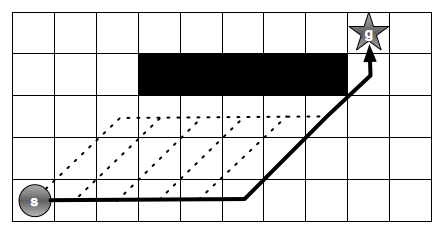
\includegraphics[scale=0.36]{diagrams/symmetry_example.png}
       \end{center}
       \caption{A pathfinding instance with high symmetry. We highlight the
eventual solution returned by A* (strong line) and a number of symmetric 
alternatives (dashed lines).}
       \label{fig-symmetry}
		\vspace{-0.5em}
\end{figure}

We begin by making precise the notion of a symmetric relationship between paths
in a uniform cost graph:
\begin{definition}
Two paths $\pi_{1}$ and $\pi_{2}$ are symmetric if they share the same start and
goal node and one can be derived from the other by interchanging the order of the
moves.
\end{definition}

Consider the pathfinding instance illustrated in Figure \ref{fig-symmetry}.
There are many symmetrical paths, some of which are marked in the figure.  With
the popular Octile heuristic in use (which is analogous to Manhattan distance,
but optimised for 8-connected grids) most nodes along symmetrical optimal paths
have an $f$ value smaller than the $f$ value of the goal.  Running A* on the
original grid will needlessly expand all such nodes.  We address this problem by
employing the following high-level strategy to identify and eliminate path
symmetries from 4 and 8-connected uniform cost grid maps:
\input alg_rsr

Our approach has similarities with the one used by
\cite{harabor10}.  The main differences are: (i) a
generalisation of the empty rectangles method to allow optimal traversal in
8-connected grid maps (ii) an offline pruning operator for reducing the size of
a rectangle's perimeter and (iii) a new online pruning strategy that allows faster
node expansion and further speeds up search.

The generalisation to uniform-cost 8-connected grids is more challenging than it might look
at a first glance.  On a 4-connected map no node requires more than one
macro-edge (to the closest node on the opposite side of the perimeter) to retain
optimality~\cite{harabor10}.  Thus, it is easy to maintain a low branching
factor.
As we show in the next section, many more macro-edges are
needed to preserve optimality on 8-connected maps. We will identify a set of
macro-edges that is necessary and sufficient to ensure that empty rectangles can
be crossed optimally.  Keeping the branching factor within reasonable limits is
a primary motivation for the enhancements reported in the next sections.

